\documentclass[10pt]{book}

%These tell TeX which packages to use.
\usepackage{array,epsfig}
\usepackage{amsmath}
\usepackage{amsfonts}
\usepackage{amssymb}
\usepackage{amsxtra}
\usepackage{amsthm}
\usepackage{mathrsfs}
\usepackage{color}
\usepackage{enumitem}

\usepackage{pgfplots}
\pgfplotsset{compat=1.6}

\pgfplotsset{soldot/.style={color=black,only marks,mark=*}} \pgfplotsset{holdot/.style={color=black,fill=white,only marks,mark=*}}

%Here I define some theorem styles and shortcut commands for symbols I use often
\theoremstyle{definition}
\newtheorem{defn}{Definition}
\newtheorem{thm}{Theorem}
\newtheorem{cor}{Corollary}
\newtheorem*{rmk}{Remark}
\newtheorem{lem}{Lemma}
\newtheorem*{joke}{Joke}
\newtheorem{ex}{Example}
\newtheorem*{soln}{Solution}
\newtheorem{prop}{Proposition}

\newcommand{\lra}{\longrightarrow}
\newcommand{\ra}{\rightarrow}
\newcommand{\surj}{\twoheadrightarrow}
\newcommand{\graph}{\mathrm{graph}}
\newcommand{\bb}[1]{\mathbb{#1}}
\newcommand{\Z}{\bb{Z}}
\newcommand{\Q}{\bb{Q}}
\newcommand{\R}{\bb{R}}
\newcommand{\C}{\bb{C}}
\newcommand{\N}{\bb{N}}
\newcommand{\M}{\mathbf{M}}
\newcommand{\m}{\mathbf{m}}
\newcommand{\MM}{\mathscr{M}}
\newcommand{\HH}{\mathscr{H}}
\newcommand{\Om}{\Omega}
\newcommand{\Ho}{\in\HH(\Om)}
\newcommand{\bd}{\partial}
\newcommand{\del}{\partial}
\newcommand{\bardel}{\overline\partial}
\newcommand{\textdf}[1]{\textbf{\textsf{#1}}\index{#1}}
\newcommand{\img}{\mathrm{img}}
\newcommand{\ip}[2]{\left\langle{#1},{#2}\right\rangle}
\newcommand{\inter}[1]{\mathrm{int}{#1}}
\newcommand{\exter}[1]{\mathrm{ext}{#1}}
\newcommand{\cl}[1]{\mathrm{cl}{#1}}
\newcommand{\ds}{\displaystyle}
\newcommand{\vol}{\mathrm{vol}}
\newcommand{\cnt}{\mathrm{ct}}
\newcommand{\osc}{\mathrm{osc}}
\newcommand{\LL}{\mathbf{L}}
\newcommand{\UU}{\mathbf{U}}
\newcommand{\support}{\mathrm{support}}
\newcommand{\AND}{\;\wedge\;}
\newcommand{\OR}{\;\vee\;}
\newcommand{\Oset}{\varnothing}
\newcommand{\st}{\ni}
\newcommand{\wh}{\widehat}
%Pagination stuff.
\setlength{\topmargin}{-0.75in}
\setlength{\oddsidemargin}{0in}
\setlength{\evensidemargin}{0in}
\setlength{\textheight}{9.in}
\setlength{\textwidth}{6.5in}
\pagestyle{empty}
\begin{document}
\begin{flushleft}
Name:\underline{\hspace{13cm}}Date:\underline{\hspace{2cm}}
\end{flushleft}
\begin{center}
{\Large Math 1041-012 \hspace{0.5cm} Quiz \#1}
\end{center}
\vspace{0.2 cm}
\subsection*{Problem 1}The displacement (in feet) of a certain particle moving in a straight line is given by $s(t)=2t^2+1$, where $t$ is measured in seconds. Find the average velocity over the following time intervals:
\begin{enumerate}[label=(\alph*)]
    \item $[1,4]$\\ \vspace{1.5cm}
    \item $[1,2]$\\ \vspace{1.5cm}
    \item $[1,1.5]$\\ \vspace{1.5cm}
\end{enumerate}
\subsection*{Problem 2} The following table gives values of $f(x)$ for values of $x$ close to $2$, but not equal to $2$:
\begin{figure}[h!]
    \centering
    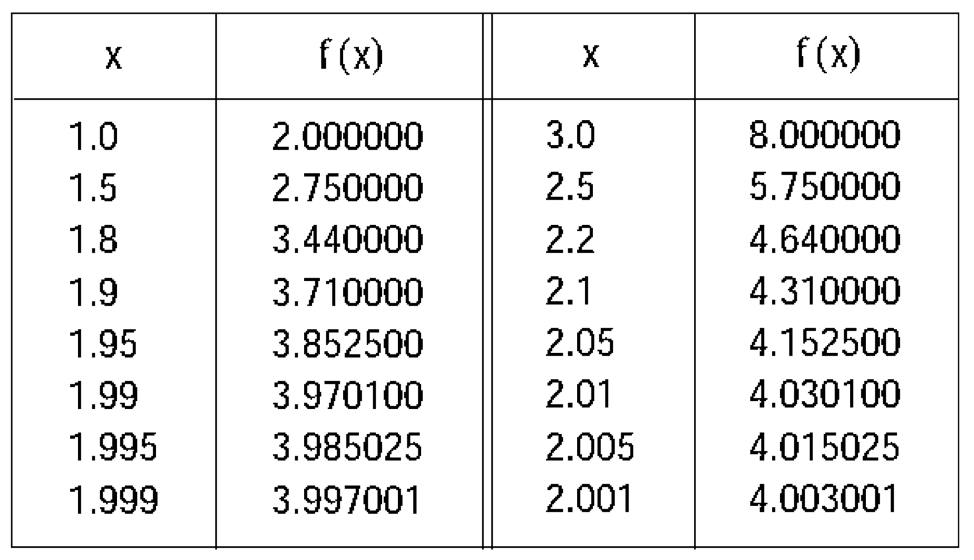
\includegraphics[scale=0.45]{fig1.png}
\end{figure}
\begin{itemize}
    \item[(a)] Estimate $\displaystyle\lim_{x\rightarrow 2^-}f(x)$
    \item[(b)] Estimate $\displaystyle\lim_{x\rightarrow 2^+}f(x)$
    \item[(c)] Does $\displaystyle\lim_{x\rightarrow 2}f(x)$ exist? Explain!
\end{itemize}
\raggedbottom
\clearpage
\subsection*{Problem 3}
Use the plot of $f(x)$ below, to evaluate the limits.
\begin{center}
\begin{tikzpicture}
\begin{axis}[
  axis x line=middle, axis y line=middle,
  ymin=-4, ymax=6, ytick={-3,...,6}, ylabel=$y$,
  xmin=-6, xmax=11, xtick={-6,...,10}, xlabel=$x$,
  axis line style={<->}, width=12cm,height=8cm
]
\addplot[domain=-2:2,black] {x*x-1};
\addplot[domain=2:6,black] {5-x};
\addplot[<-,domain=-6:-2,black] {-3};
\addplot[->,domain=6:10,black]{1/(x-6)};
\draw[dashed] (axis cs:6,6) -- (axis cs:6,-5);
\addplot[holdot] coordinates{(-2,-3)(-2,3)(2,3)};
\addplot[soldot] coordinates{(-2,1)(2,4)(6,-1)};
\end{axis}
\end{tikzpicture}
\end{center}
\begin{alignat*}{3}
&\lim_{x\rightarrow -2^-}f(x)\hspace{2cm} &&  \lim_{x\rightarrow -2^+}f(x)\hspace{2cm} && \lim_{x\rightarrow -2}f(x)\\[8pt]
&\lim_{x\rightarrow 2^-}f(x)\hspace{2cm} &&  \lim_{x\rightarrow 2^+}f(x)\hspace{2cm} && \lim_{x\rightarrow 2}f(x)\\[8pt]
&\lim_{x\rightarrow 6^+}f(x)\hspace{2cm} &&  \lim_{x\rightarrow 6^-}f(x)\hspace{2cm} && \lim_{x\rightarrow 0}f(x)\\[8pt]
&\lim_{x\rightarrow 1}f(x) && \lim_{x\rightarrow -1^-}f(x) &&\lim_{x\rightarrow 6}f(x)
\end{alignat*}
\raggedbottom
\end{document}